
\subsection{Power Supply}
The power supply has been build to deliver 3 different voltage levels (5V, 6V, 12V), ensuring a current of 1A, 1.5A and 1A respectively.

This circuit has been printed in a PCB that can be plugged directly in a breadboard to deliver the required voltage and current.

The power supply is conected to a 15V power supply as a input voltage. To convert this 15V into 12V, 6V and 5V 3 different elements are used.

To ensure a 5V/1A supply with a +-1.5\% voltage for the FPGA, an LM2574 regulator is used. 

About the 6V/1.5A and 12V/1A, the 7806 and 7812 regulators are used. As the efficiency of these regulators is not as good as the one of the LM2574 and they dissipate the excess of power by heating up, a heatsink for the 


\begin{figure}[H]
\centering 
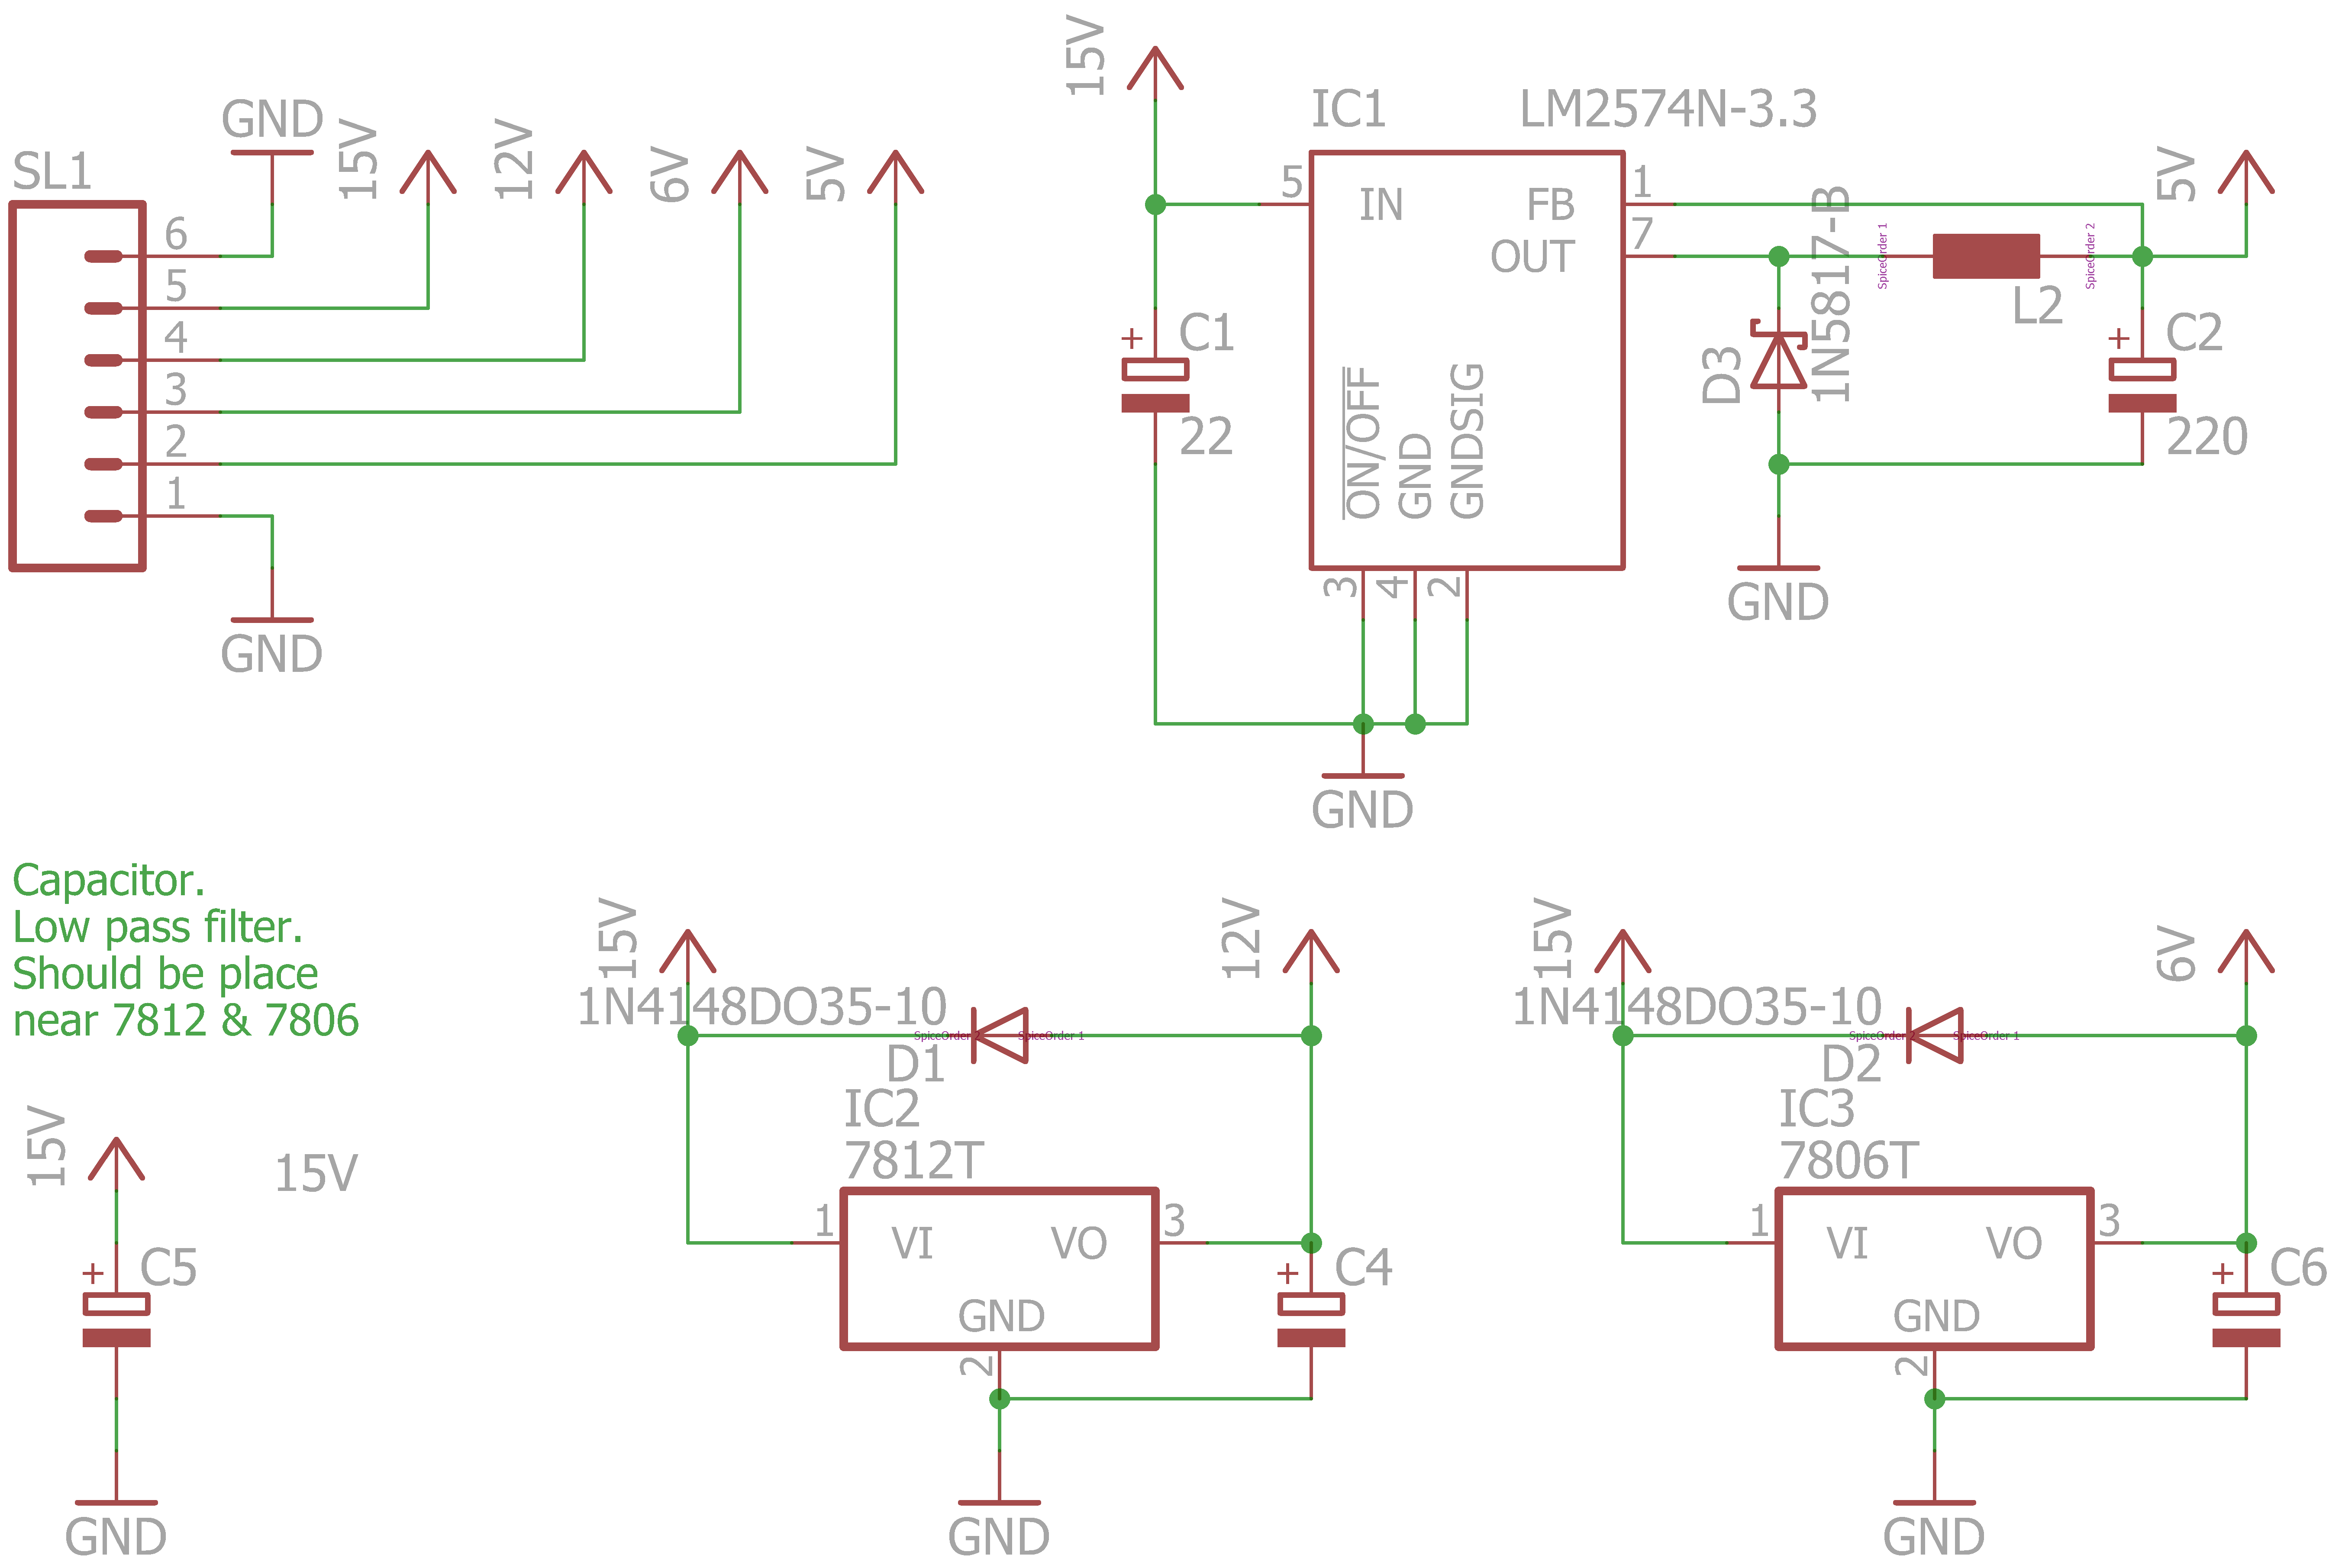
\includegraphics[width = 0.4 \textwidth]{images/powersupply_schematics}
\caption{...}
\label{fig:...}
\end{figure}